\chapter{Ændring af Konteksten}
Som der beskrives i den initierende problemstilling, er det vanskeligt at vedligeholde trafikmodeller, på grund de ændringer der sker i konteksten. Disse ændringer er fundet til at være en vækst i bestanden af køretøjer, og et skift i hvilke transportmidler der bliver benyttet af Danskere.

\vspace{5mm}

Data fra Danmarks Statistik viser en vækst i bestanden af køretøjer som ses på figur \ref{plotvaekstbiler}. I tilfælder hvor en trafikmodel ikke tager denne vækst med i overvejelserne, kan det føre til et urealistisk billede af virkeligheden, i det at der sandsynligvis vil være mindre stress på vejnettet.

\vspace{5mm}

Hvis man sammenligning antallet af køretøjer med befolkningsantallet, vil man se en stigning i køretøjer per borger. I 1995 var der et køretøj til 41\% af borgerne, og i 2016 er dette steget til et køretøj til 55\% af borgerne. For trafikmodeller der kun undersøger afviklingen af biltrafik vil dette ikke have nogen påvirkning, men for modeller der inddrager andre transportmidler vil dette skift skulle tages med i beregningerne, hvis der bliver kigget på fremtiden.

\begin{figure}[h!]
    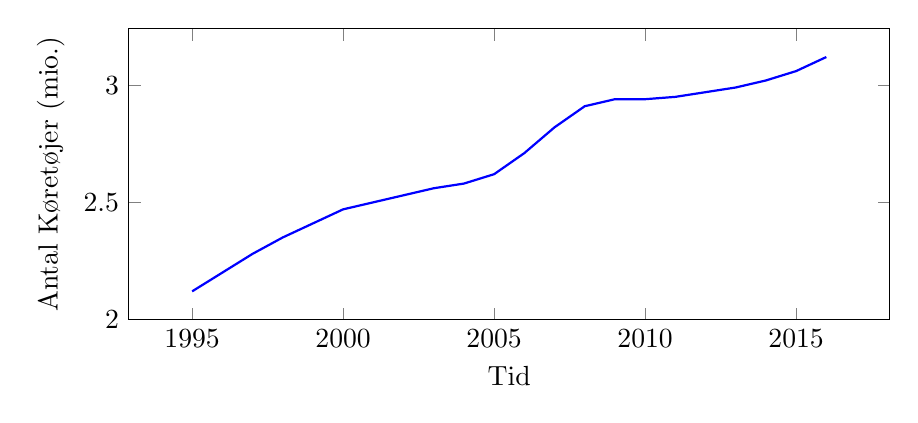
\begin{tikzpicture}
    \begin{axis}
	[
	    xlabel=Tid, 
	    ylabel=Antal Køretøjer (mio.), 
	    ymin=2, 
	    ymax=3.24,
	    width=320,
	    height=150,
	    x tick label style={/pgf/number format/1000 sep=} % Fjerner komma i Året
    ]
    \addplot[blue, thick] coordinates 
    {
        (1995, 2.12)
    	(1996, 2.20)
    	(1997, 2.28)
	    (1998, 2.35)
	    (1999, 2.41)
	    (2000, 2.47)
	    (2001, 2.50)
    	(2002, 2.53)
    	(2003, 2.56)
    	(2004, 2.58)
    	(2005, 2.62)
    	(2006, 2.71)
    	(2007, 2.82)
    	(2008, 2.91)
    	(2009, 2.94)
	    (2010, 2.94)
	    (2011, 2.95)
	    (2012, 2.97)
	    (2013, 2.99)
    	(2014, 3.02)
    	(2015, 3.06)
    	(2016, 3.12)
    };
    \end{axis}
\end{tikzpicture}
    \caption{Væksten i bestanden af køretøjer}
    \label{plotvaekstbiler}
\end{figure}

% Bestanden af biler kilde: http://www.statistikbanken.dk/BIL8
% Befolkningstal kilde: http://www.statistikbanken.dk/HISB3

\section{Transportmiddelvalg}
Det kan argumenteres, baseret på vedligeholdelsesparametre angivet heri at baggrunden for en trafikmodel der kan være fremtidigt brugbar afhænger af andre tilfælde end lige netop befolkningsantal. Det kan også anskues at andre herunder givne parametre kunne gøre simulering af disse trafikmodeller en vanskelighed, hvori en drastisk ændring kunne medføre grunde til fejlkilder ved vedligeholdelse af de førhen nævnte modeller.

\begin{itemize}
\item Transportmidlers popularitet
\item Ny teknologi
\item Adfærd
\end{itemize}

Under disse parametre kan der uddrages en række kategorier af transportmidler der er gældende for trafikmodellerne, dette kan også forstås som alle nuværende relevante transportmidler for persontransport. Disse kan lægges under kategorierne kollektiv transport (busser, toge mm.) og personlig transport (personbiler, cykler mm.)

\vspace{5mm}

Transportmidlers popularitet kunne indebære en stigning i behovet for at benytte cykler eller lignende. Denne parameterændring ville være et essentiel eksempel at bearbejde til at videregive en bedre vedligeholdelsesstandard, antaget at der findes grundlag for dette.

\vspace{5mm}

Ny teknologi indebærer forbedringer til nuværende transportmuligheder og integration med nuværende orienteringsværktøjer som f.eks. applikationer. Simulering af denne parameterændring er uforudsigelig i bedste tilfælde, dog kan undersøgelser henligge til mulig nye teknologier der kunne have relevans.

\vspace{5mm}

Adfærdsmønstre er lige så uforudsigelige hvis ikke mere end nye teknologier. Heri består samfundsændringer der afgører landskabet som trafikmodellerne håndterer osv.

\vspace{5mm}

Ud fra disse kategorier er der udvalgt en række transportmidler. Transportmidlerne er baseret på kategoriernes prioritet i forhold til relevans for løsningsmodellen. Kollektive og personlige transportmidler kan stilles op foran hinanden og argumenteres på baggrund af forudsigelige ændringer i parametre. Herunder grundlaget beliggende i væksten af priser mellem de forskellige transportmuligheder og parameterændringer for på et samfundsmæssigt og teknologisk grundlag.